\chapter{Application Layer}
\label{chapter:applicationlayer}

% OVERVIEW
\section{Overview}
This section gives an overview over the components of the applacation layer (GUI) of ACE. Figure \ref{applicationlayer_ace_overview} shows the graphical user interface (GUI) with all components. Each component is explained detailed in section \ref{applicationlayer_components}.
\begin{figure}[H]
\begin{center}
  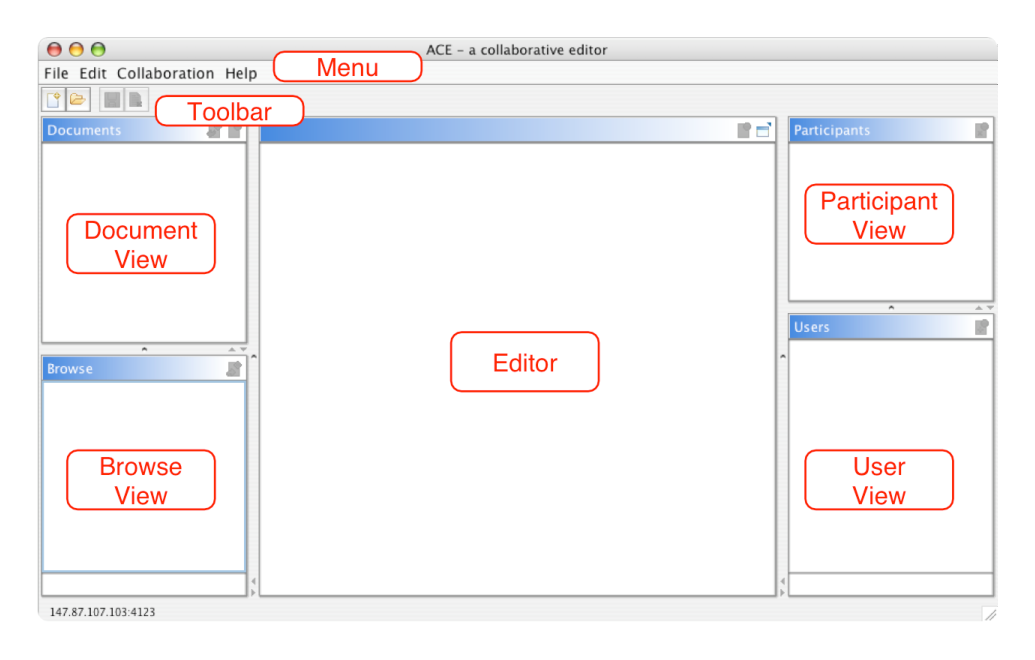
\includegraphics[height=3.135in, width=5.01in]{../images/finalreport/application_ace_overview.eps}
\caption{ACE Overview}
\label{applicationlayer_ace_overview}
\end{center}
\end{figure}
On the top of the application are the menubar and the toolbar. The menubar is splitted into four menus which are containing functions associated to their category. Below the menubar is the toolbar that contains the most used functions out of the menu.

In the middle of the GUI are the four views and the editor component. The document view shows the current opened documents, the browse view contains all documents that can be found over the network (published by other users), the user view shows all users running ACE in the same network and the participant view contains a list of all users that are currently editing in the selected document.

At the bottom of the application is the status bar that simple contains a label which dispays the current IP address.

% COMPONENTS
\section{Components}
\label{applicationlayer_components}

% FRAME
\subsection{Frame}
The main frame of the application layer is based in a \texttt{PersistentFrame} (not yet full implemented). A persistent frame is a simple \texttt{JFrame} that saves the last position and size. Each time an application is started, the frame has the same position like last time before the application has terminated. Its possible to set a \textit{JMenuBar}, a \textit{JToolBar}, a status bar \textit{JPanel} and the content (\textit{JPanel}). Further, the \texttt{PersistentFrame} has a \textit{windows listener} to catch the windows closing event and forward it to an \textit{exit action}.

% MENU
\subsection{Menu}
The menu of the application layer is basically a \textit{JMenuBar} containing \textit{JMenu} entries. Each \textit{JMenu} has one or more \textit{AbstractAction} and \textit{JSeparator}. The following figure illustrates how it is built up:
\begin{figure}[H]
\begin{center}
  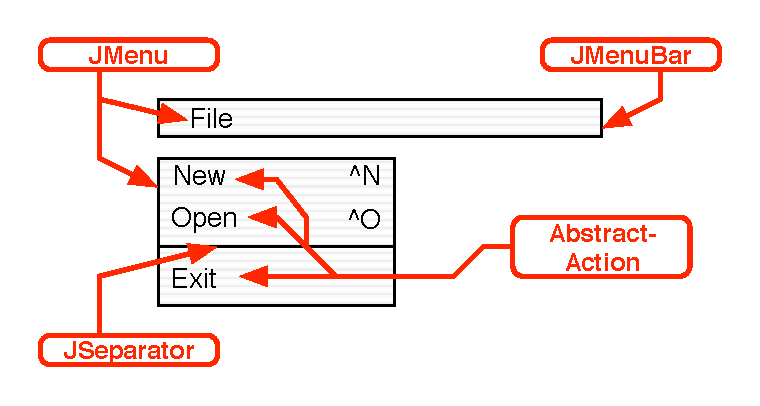
\includegraphics[height= 2.08in, width= 4.85in]{../images/finalreport/application_menu.eps}
\caption{Collaborative Editor Class Diagram}
\label{application_menu}
\end{center}
\end{figure}
This menu is created by the method \texttt{createMenuBar()} in the \textit{ApplicationFactory} (see section \ref{applicationlayer_applicationfactory}):
\begin{verbatim}
  public JMenuBar createMenuBar() {
    JMenuBar menuBar = new JMenuBar();

    JMenu m1 = new JMenu("Menu 1");
    m1.add(...);        // add actions for menu 1
    menuBar.add(m1);    // add menu 1 to the menubar
    
    JMenu m2 = new JMenu("Menu 2");
    m2.add(...);        // add actions for menu 2
    menuBar.add(m2);    // add menu 2 to the menubar
    
    return menuBar;
  }
\end{verbatim}

% TOOLBAR
\subsection{Toolbar}
Toolbars are used to make the most used functions (actions) comfortably operated. The application layer uses a \textit{JToolBar} for this purpose. Its created by the \textit{ApplicationFactory} in the method \textit{createToolBar()}:
\begin{verbatim}
  public JToolBar createToolBar() {
    JToolBar toolBar = new JToolBar();
    toolBar.setFloatable(false);   // make it impossible to drag the toolbar
    toolBar.setRollover(true);

    toolBar.add(...);   // add actions to toolbar

    return toolBar;
  }
\end{verbatim}

% VIEWS
\subsection{Views \& View Controllers}
This section gives an overview of all the used \textit{views} and how they are managed by the \textit{view controllers}. The figure \ref{application_views_controllers} show the class diagram from the view's and the controller's. NOTE: the shortcut \textit{ISC} stands for \textit{ItemSelectionChange}.
\subsubsection{Overview}
\begin{figure}[H]
\begin{center}
  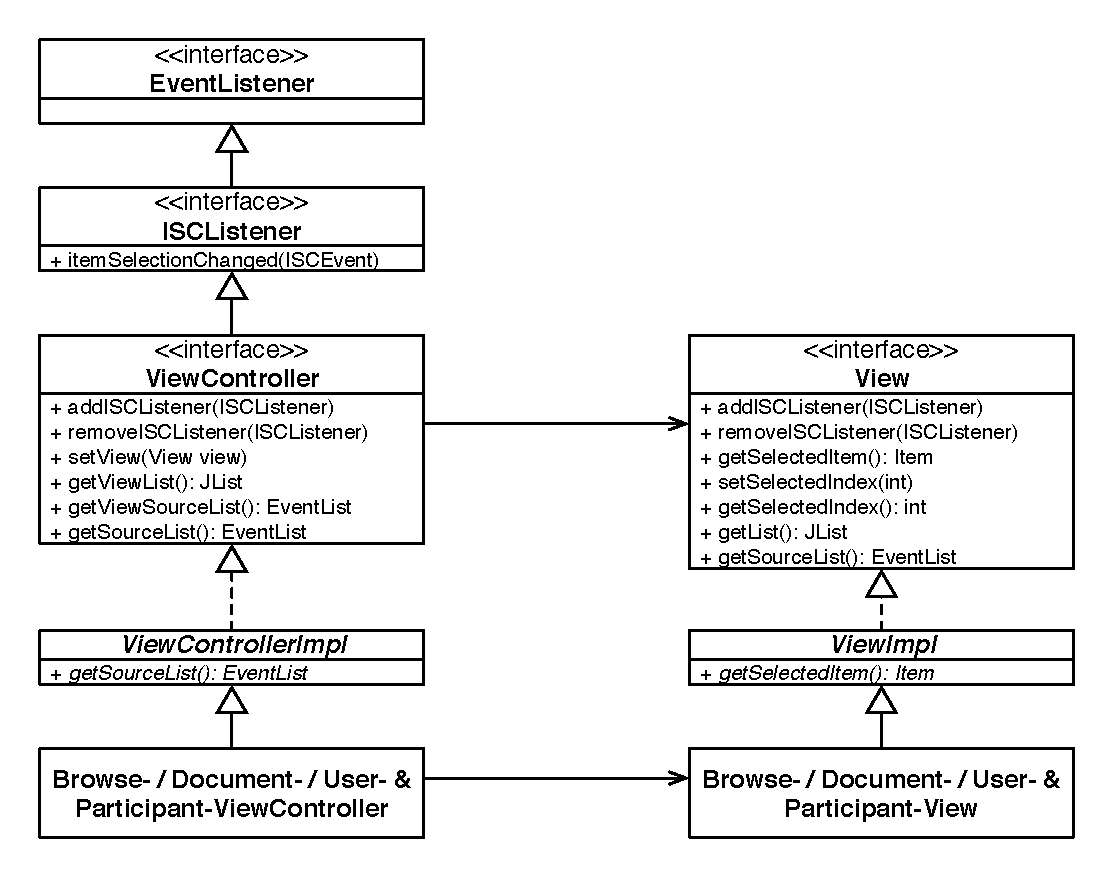
\includegraphics[height=5.62in, width=7.19in]{../images/finalreport/application_views_controllers.eps}
\caption{Collaborative Editor Class Diagram}
\label{application_views_controllers}
\end{center}
\end{figure}
Each view has its own controller (e.g. a \textit{BrowseView} has a \textit{BrowseViewController}). View controllers are managing the data source of the views and are needed to insert, remove or replace elements. The view only displays the elements from the data source. Moreover, a view returns the current selected element to the view controller. The construction of the view and the corresponding controller needs the following steps:
\begin{enumerate}
\item create the view controller
\item create the view (code fragment from the contructor of \texttt{ViewImpl}):
  \begin{verbatim}
    public ViewImpl(ViewController controller, ...) {
      controller.setView(this);
      addItemSelectionChangeListener(controller);
    }
  \end{verbatim}
  After the view has been created, the the view is registered by its controller (\texttt{controller.setView(this)}) and the controller receives the \texttt{ItemSelectionChangeEvent} if the selection has changed on the view.
\end{enumerate}
To keep the displayed list elements up to date \textit{Glazed Lists} (see section \ref{appendix_frameworks_glazedlists} for more details) are used. \textit{Glazed Lists} providing \textit{EventLists} which are observing their elements. If such an element changes a property (and fires a \texttt{firePropertyChange(...)}) the list will automatically be updated and you dont have to care about that yourself.

The next sections are giving an overview of details from the four different views.

\subsubsection{Document View \& Controller}
The document view is used to display the current open documents. A current open document can either be a local document (new or existing document on the local machine), a published document (a local document that has been published) or a joined document published by another user. All needed information for documents are nested into \textit{DocumentItems}. The most important attributes of document items are:
\begin{itemize}
\item Type: the type decides for what kind of document the document item is needed (e.g. local, published, remote, joined document).
\item Editor Document: the styled document (see section \ref{applicationlayer_collabdocument}) that is displayed in the text component.
\item If the type is remote or shared: the \textit{Session} and \textit{SessionCallback} are referenced to send and receive \textit{Operations}.
\end{itemize}
\begin{figure}[H]
\begin{center}
  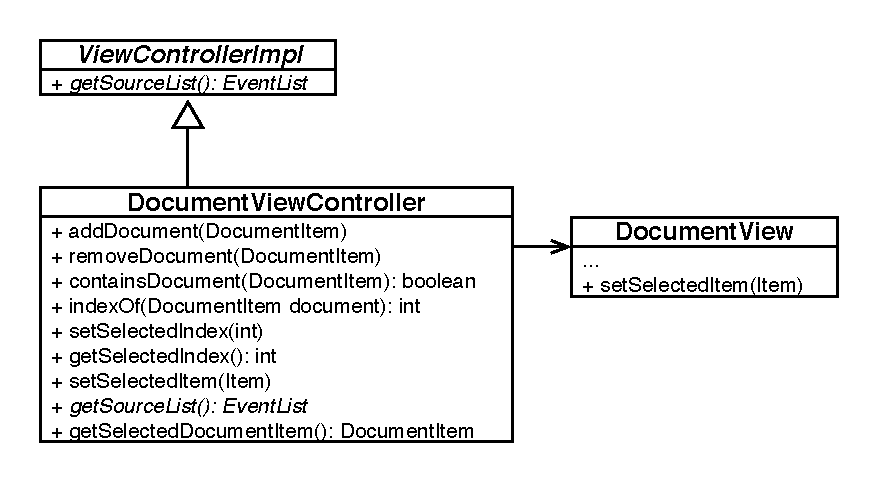
\includegraphics[height=2.99in, width=5.62in]{../images/finalreport/application_documentview.eps}
\caption{Document View Controller}
\label{application_documentview}
\end{center}
\end{figure}
The \textit{DocumentItem} class is used for other document types than \textit{local}, \textit{published} or \textit{joined} too. To display only the documents with these types, a so called \textit{Matcher} is needed:
\begin{verbatim}
  Matcher documentViewMatcher = new Matcher() {
    public boolean matches(Object item) {
      DocumentItem dItem = (DocumentItem)item;
      return (dItem.getType() == DocumentItem.LOCAL ||
      dItem.getType() == DocumentItem.PUBLISHED ||
      dItem.getType() == DocumentItem.JOINED);
    }
  };
\end{verbatim}
This matcher is filtering the source list containing all document items and returns only the document items with the corresponding type.

\subsubsection{Browse View \& Controller}
The browse view displays all documents that are published by other users in the same network. The browse view controller that controls the browse view implements a \textit{DocumentListener} that notifes the controller whenever new documents have been found on the network or existing document have been discarded.
\begin{figure}[H]
\begin{center}
  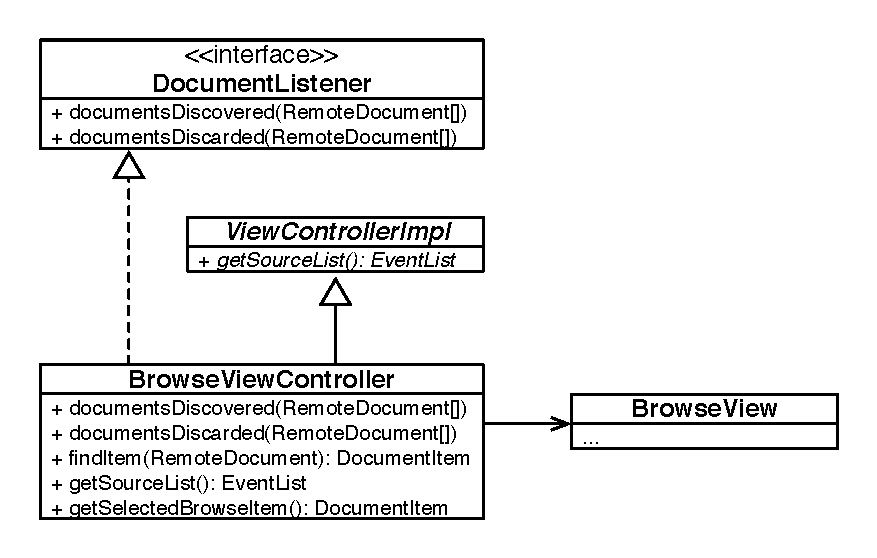
\includegraphics[height=3.5in, width=5.62in]{../images/finalreport/application_browseview.eps}
\caption{Browse View Controller}
\label{application_browseview}
\end{center}
\end{figure}

Because the browse view uses the same source list of document items than the document view, another filter (matcher) is needed to separate the documents after their types. The browse view only displays documents of the types remote and waiting. A document item has the type awaiting while joining a remote document.
\begin{verbatim}
  Matcher browseViewMatcher = new Matcher() {
    public boolean matches(Object item) {
      DocumentItem dItem = (DocumentItem)item;
      return (dItem.getType() == DocumentItem.REMOTE ||
      dItem.getType() == DocumentItem.AWAITING);
    }
  };
\end{verbatim}
In case that there are a lot of users with a lot of published documents in a network the browse view has a filter. This filter allows the user to type a publisher name into a textfield. All documents that are not from this publisher will be removed from the list:
\begin{verbatim}
  JTextField browseFilterField = new JTextField();
  TextFilterator browseFilterator = new TextFilterator() {
    public void getFilterStrings(List baseList, Object element) {
      DocumentItem item = (DocumentItem)element;
      baseList.add(item.getPublisher());
    }
  };
\end{verbatim}

\subsubsection{User View \& Controller}
The user view displays all other users running ACE in the same local area network. The user controller receives a notification from the \textit{UserListener} whenever a user has been discovered or discarded. On this way he manages the list of users the \textit{User View} is displaying.
\begin{figure}[H]
\begin{center}
  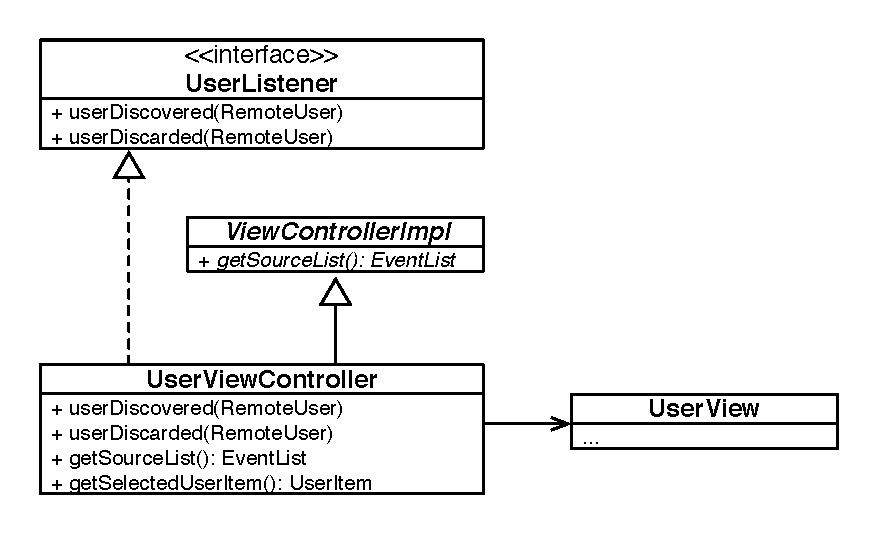
\includegraphics[height=3.33in, width=5.62in]{../images/finalreport/application_userview.eps}
\caption{User View Controller}
\label{application_userview}
\end{center}
\end{figure}
For finding fast a single user out of the rest the \textit{User View} has a filter. The filter is based on the text entered into a textfield and compares that to the usernames:
\begin{verbatim}
  JTextField userFilterField = new JTextField();
  TextFilterator userFilterator = new TextFilterator() {
    public void getFilterStrings(List baseList, Object element) {
      UserItem item = (UserItem)element;
      baseList.add(item.getName());
    }
  };
\end{verbatim}

\subsubsection{Participant View \& Controller}
At the moment a document is published, a list of participants i created. At the beginning only the publisher himself is in this list.  For each user joining the document, a new \textit{ParticipantItem} is created and added to the list. The \textit{ParticipantItem} contains the name of the participant and the color needed to highlight his text. The \textit{Participant View} displays all these \textit{ParticipantItems} of a session.
\begin{figure}[H]
\begin{center}
  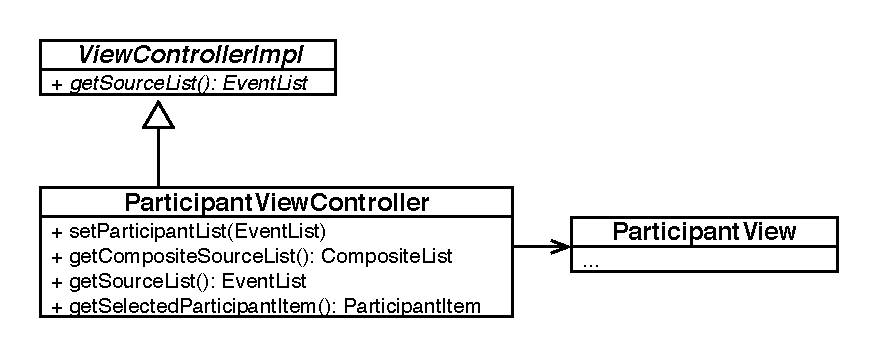
\includegraphics[height=2.15in, width=5.62in]{../images/finalreport/application_participantview.eps}
\caption{Participant View Controller}
\label{application_participantview}
\end{center}
\end{figure}
Each published document has its own list of participants which needs to be set in the \textit{Participant View Controller} when the current displayed document changes.
\begin{verbatim}
  public void setParticipantList(EventList participantList) {
    // remove old participant list if there is one
    if (memberList != null) {
      participantSourceList.removeMemberList(memberList);
    }

    // add new participant list    
    this.memberList = participantList;
    participantSourceList.addMemberList(participantList);
  }
\end{verbatim}

% ACTIONS
\subsection{Actions}
All actions used by the application layer are subclasses of the java \textit{AbstractAction}. They have a \textit{name}, an \textit{icon} and optional a \textit{shortcut} and a \textit{tooltip}. The \textit{name} and the \textit{icon} can be forwarded to the superclass, how to set the \textit{shortcut} and the \textit{tooltip} is shown in the following code fragment:
\begin{verbatim}
  // somewhere in costructor (shortcut = CTRL + X)
  putValue(ACCELERATOR_KEY, KeyStroke.getKeyStroke('X',
    Toolkit.getDefaultToolkit().getMenuShortcutKeyMask()));

  putValue(SHORT_DESCRIPTION, "Tooltip text here...");
\end{verbatim}
Most of the actions are depending on the selection of the \textit{Document View}. This leads to the \textit{DocumentItemSelectionChangeAction} class:
\begin{figure}[H]
\begin{center}
  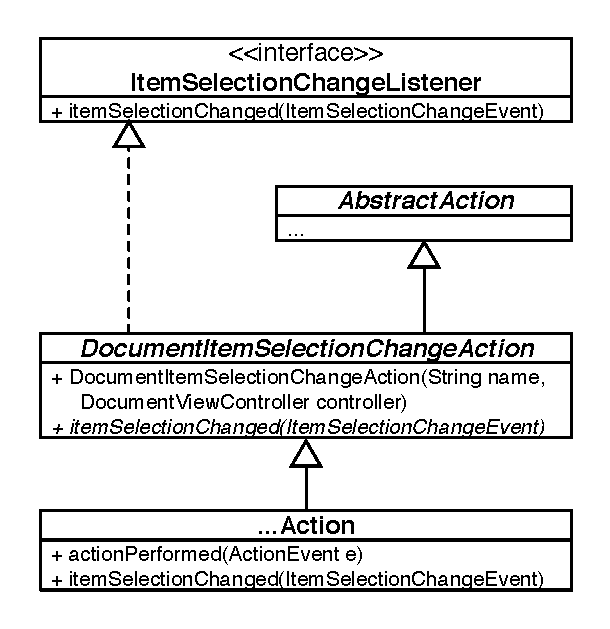
\includegraphics[height=3.97in, width=3.85in]{../images/finalreport/application_action.eps}
\caption{DocumentItemSelectionChangeAction Class Diagramm}
\label{application_application_action}
\end{center}
\end{figure}
This class handles the registration of the action to the \textit{ItemSelectionChangeListener} of  the \textit{Document View Controller}.
\begin{verbatim}
  public abstract class DocumentItemSelectionChangeAction
    extends AbstractAction implements ItemSelectionChangeListener {
  
    public DocumentItemSelectionChangeAction(String name, Icon icon,
          DocumentViewController viewController) {
      super(name, icon);
      viewController.addItemSelectionChangeListener(this);
    }
    
    public abstract void itemSelectionChanged(ItemSelectionChangeEvent e);
  }
\end{verbatim}



% EDITOR
\subsection{Editor}
This section gives an overview of all components needed for the collaborative editor. The following figure shows the class diagram:
\begin{figure}[H]
\begin{center}
  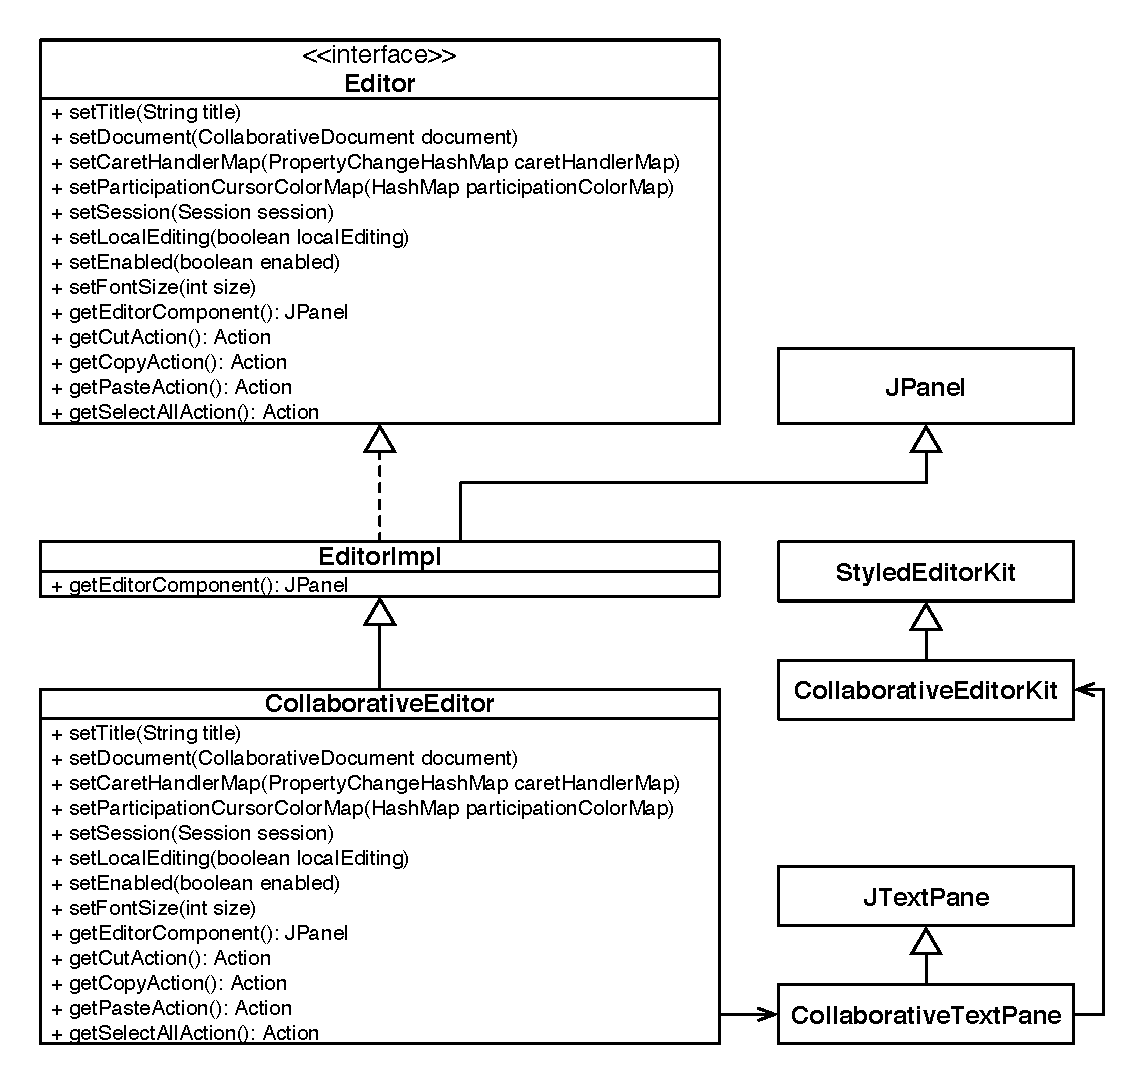
\includegraphics[height=5.25in, width=5.55in]{../images/finalreport/application_editor.eps}
\caption{Collaborative Editor Class Diagram}
\label{application_editor}
\end{center}
\end{figure}

\subsubsection{Collaborative Editor}
The collaborative editor is a JFrame which support all functionality defined in the \textit{Editor} interface. The constructor looks like:
\begin{verbatim}
  public CollaborativeEditor(...) {
    // create editor pane & kit
    cTextPane = new CollaborativeTextPane();
    cEditorKit = new CollaborativeEditorKit();
    cTextPane.setEditorKit(cEditorKit);

    // create editor pane
    JScrollPane scrollPane = new JScrollPane(cTextPane);
    editorPane = new SimpleInternalFrame(null, " ", editorToolBar, scrollPane);

    // add components		
    setLayout(new BorderLayout());
    add(editorPane);    
  }
\end{verbatim}

All setter methods (except \texttt{setTitle(...)} that sets directly the tilte of the frame) are directly forwarded to the collaborative text pane (\texttt{cTextPane}) like:
\begin{verbatim}
  public void setXYZ(...) {
    cTextPane.setXYZ(...);
  }
\end{verbatim}

To use the standard text component actions for the menu \textit{edit}, we need getter methods that returns them. All text component actions are handled in the editor kit (see section \ref{collaborative_editor_kit}), thus we forward the getter methods to the collaborative editor kit (\texttt{cEditorKit}):
\begin{verbatim}
  public Action getXYZAction() {
    return cEditorKit.getXYZAction();
  }
\end{verbatim}



\subsubsection{Collaborative TextPane}
The collaboration text pane implements all functionality defined by the \texttt{Editor} interface. This component overrides the \texttt{replaceSelection} method from its superclass \texttt{JTextPane}. This is needed to use a lock while inserting content into the document. Locking has to be done to avoid asynchronous text insertions while creating and sending operations that are based on the document content.
\begin{verbatim}
  public void replaceSelection(String content) {
    SessionTemplate template = new SessionTemplate(session);
    template.execute(new SessionTemplateCallback() {
      public void execute(Session session) {

        // create and send operation
        Operation op  = new Delete/InsertOperation(...);
        session.sendOperation(op);

        // call superclass method
        CollaborativeTextPane.super.replaceSelection(content);
      }
    }
  }
\end{verbatim}
Furthermore there is a method \texttt{setCaretHandlerMap(PropertyChangeHashMap caretHandlerMap)} which is responsible to set the map with the carets (cursor positions) from all participants of the current document. The \texttt{PropertyChangeHashMap} is a map that adds a \texttt{PropertyChangeListener} on all inserted elements (carets from other users) and forwards their \texttt{PropertyChangeEvents} to all registered components. The following code fragment makes the editor able to receive updates if the carets of other users have changed:
\begin{verbatim}
  public void setCaretHandlerMap(PropertyChangeHashMap caretHandlerMap) {
    // unregister old map
    this.caretHandlerMap.removePropertyChangeListener(this);
    this.caretHandlerMap = caretHandlerMap;

    // register new map
    this.caretHandlerMap.addPropertyChangeListener(this);
  }
\end{verbatim}
To handle the own caret changes its necessary to register a \texttt{CaretListener}. The invoked method \texttt{caretUpdate(...)} checks if the current user really changed his cursor position and needs to send the new caret position to the session.

Each time a caret of another user changes the method \texttt{propertyChange(PropertyChangeEvent evt)} will be invoked. The \texttt{PropertyChangeEvent} contains the old and the new caret position from the users that moved his caret and forces a repaint. The implementation looks like:
\begin{verbatim}
  public void propertyChange(PropertyChangeEvent evt) {
    // old caret
    CaretUpdate oldCU = (CaretUpdate)evt.getOldValue();
    Rectangle oldRect = modelToView(oldCU.getDot());
    repaint(oldRect);

    // new caret
    CaretUpdate newCU = (CaretUpdate)evt.getNewValue();
    Rectangle newRect = modelToView(newCU.getDot());
    repaint(newRect);
  }
\end{verbatim}
The \texttt{repaint(...)} is eighter called by swing or explicit by the \texttt{propertyChange} method when one of the participant changed his cursor position. It iterates through the \texttt{caretHandlerMap} and paints the caret for each map entry.

\subsubsection{Collaborative EditoKit}
\label{collaborative_editor_kit}
The collaborative editor kit extends the styled editor kit and is needed for synchronisation purposes. To ensure the correct content of the text component its necessary to use lockings before sending operation for the following situations:
\begin{itemize}
\item \texttt{DeletePrevCharAction} which is called when the users presses the backspace key.
\item \texttt{DeleteNextCharAction} which is called when the users presses the delete key.
\item \texttt{CutAction} which is called when the user cuts some text out of the document.
\item Inserting Content: this issue is handled in the \textit{collaborative text pane}.
\end{itemize}

All editor actions are defined in an array that can be get by using the \texttt{getActions()} method from the superclass. The three delete actions listed above need to replaced by actions that are able to use locks. A simple solution would be:
\begin{verbatim}
  public class CollaborativeDeletePrevCharAction extends
    DefaultEditorKit.DeletePrevCharAction {
    
    public void actionPerformed(...) {
      // lock here
      super.actionPerformed(...);
      
      session.sendOperation(...)
      // unlock here
    }
  }
\end{verbatim}
Unfortunately its not possible to subclass the actions defined in the \texttt{DefaultEditorKit}. This leads to the solution to copy their implementation into the \texttt{CollaborativeEditorKit} and manipulate them. For example the \texttt{actionPerformed} method from \texttt{DeletePrevCharAction} looks like:
\begin{verbatim}
  public void actionPerformed(...) {
    SessionTemplate template = new SessionTemplate(session);
    template.execute(new SessionTemplateCallback() {
      public void execute(Session session) {

        // check whatever needed here and manipulate text component document
        document.remove(...);
        
        // create and send operation
        Operation op  = new DeleteOperation(...);
        session.sendOperation(op);

      }
    }
  }
\end{verbatim}


\subsubsection{Editor Controller}
The editor controller is registered for item selection change events from the \textit{DocumentViewController} and is used to enabled, disable and set editor values. Each time the selection is changed or the current document item changes properties, the following procedure is made:
\begin{itemize}
\item \textit{disable} the editor if no document is selected.
\item \textit{set} the \textit{document} of the selected item.
\item \textit{set} the editor \textit{title}.
\end{itemize}
Furthermore if the selected document is a published or a joined (remote) document the \textit{session} and the \textit{participant list} are set too.

\subsubsection{Collaborative Document}
\label{applicationlayer_collabdocument}
The collaborative document extends the \textit{DefaultStyledDocument}. It is used for getting write locks and applying text styles. Each time a style added to the document changes the method \texttt{reapplyStyles(...)} is called.
\begin{verbatim}
  protected void styleChanged(Style style) {
    if(!style.getName().equals("default")) {
      reapplyStyles(style);
    }
  }
\end{verbatim}

The method \texttt{reapplyStyles(...)} iterates through all the text elements from the document and checks if they are using the changed style. All elements using this style will be notified and updated. The following scenario will work now and all text elements will have the new background color:
\begin{verbatim}
  // add style
  Style myStyle = document.addStyle("myStyle", null);
  StyleConstants.setBackground(myStyle, Color.BLUE);
  
  // insert some text here
  doc.insertString(...);
  
  // change style
  StyleConstants.setBackground(myStyle, Color.RED);
\end{verbatim}

\subsubsection{AsyncCaret}
When inserting text into a text component and setting the caret position asynchronous, its possible that the caret isnt set to the correct position. Asynchronous caret update is implemented in Java 1.4 but there is no posibility to enable it (this problem is solved in Java 1.5). \texttt{AsyncCaret} is a simple copy of the standard caret class with the following constructor details:
\begin{verbatim}
  public AsyncCaret() {
    async = true;
  }
\end{verbatim}

% OTHER
\subsection{Other}
% APPLICATION FACTORY
\subsubsection{Application Factory}
\label{applicationlayer_applicationfactory}
To build the GUI (see section \ref{applicationlayer_wf_startup}) the \textit{Application Factory} is needed besides of \textit{Spring} (see section \ref{appendix_frameworks_spring}). It provides methods to create the \textit{Menu Bar}, the \textit{Tool Bar}, the \textit{Persistant Component Pane} and the \textit{Status Bar}.

% APPLICATION CONTROLLER
\subsubsection{Application Controller}
All functions that may need to show a dialog for user inputs or for error displaying are handled within the \textit{Application Controller}. Some functions like for example \texttt{closeDocument()} need to do some checks before they open a dialog and other functions like \textit{showAbout()} directly popup the required dialog. To show dialogs the \textit{Dialog Controller} (\ref{applicationlayer_dialogcontroller}) is used.

% DIALOG CONTROLLER
\subsubsection{Dialog Controller}
\label{applicationlayer_dialogcontroller}

% PERSISTENT CONTENT PANE
\subsubsection{Persistent Content Pane}
The \textit{Persistent Content Pane} is the container for all \textit{Views} and the \textit{Editor} component. It is a \textit{JPanel} containing several \textit{split panes} to make the GUI components resizable (see figure \ref{application_splitpane}).
\begin{figure}[H]
\begin{center}
  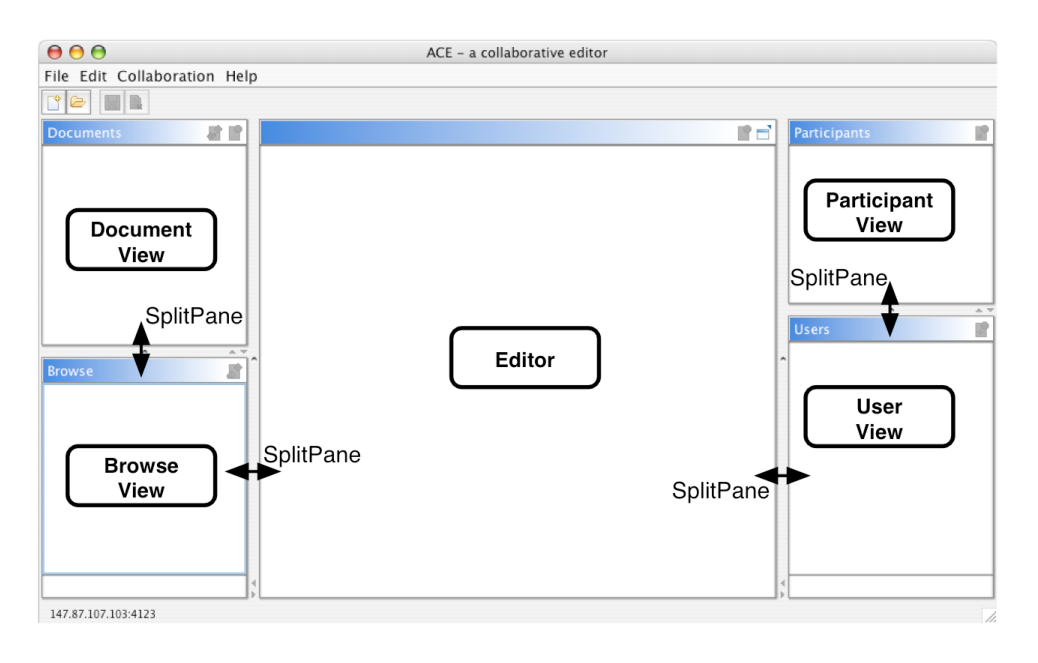
\includegraphics[height=4.19in, width=6.69in]{../images/finalreport/application_splitpane.eps}
\caption{Persistent SplitPane}
\label{application_splitpane}
\end{center}
\end{figure}
The special method \texttt{switchFullScreenEditing()} maximizes the \textit{Editor} and minimizes all other components. For the usage of this feature see \textit{User Manual, Section Editor}.



\newpage
% WORKFLOWS
\section{Workflows}

% STARTUP
\subsection{Startup}
\label{applicationlayer_wf_startup}
All the startup processes for ACE are defined in the main method from the class \textit{Main.java}:
\begin{description}
\item[1. Load Customizer ] The first step is to get the customizers. Customizers are used to create operating system based stuff like setting the look \& feel of the application.
\item[2. Load ApplicationContext ] After the customizer has been loaded, the spring application context (see \ref{appendix_frameworks_spring} for more details about spring) needs to be loaded.
\item[3. Get ApplicationFactory ] The application factory is used to create all GUI components.
\item[4. Get ApplicationController ]  
\item[5. Get CollaborationService ] 
\item[6. Load PreferencesStore ]
\item[7. Create Main Frame ]
\item[8. Init PreferencesStore ]
\item[9. Init CollaborationService ]
\item[10. Create Empty Document ]
\end{description}

% ACTION ENABLING
\subsection{Enabling of Actions}
It is important for the user-friendliness to enabled or disable actions in the GUI. The enabling of most of the actions depends on selection criteria of the views. For this pupose actions can add themself to the \textit{ItemSelectionChangeListener} of a view and receiving \textit{ItemSelectionChangedEvents}.  For example the \textit{close document} action should be only enabled if a document is selected in the \textit{Document View}:
\begin{verbatim}
  // somewhere in the constructor
  documentView.addItemSelectionChangeListener(this);

  public void itemSelectionChanged(ItemSelectionChangeEvent e) {
    if(e.getItem() == null) {
      // no document is selected
      setEnabled(false);
    } else {
      // a document is selected
      setEnabled(true);
    }
  }
\end{verbatim}

